\documentclass[12pt]{article}

\setlength\parindent{0pt}
\newcommand{\myt}[1]{\textbf{\underline{#1}}}

\usepackage{mathtools}
\usepackage{amssymb}
\usepackage{graphicx}

\title{\vspace{-15ex}Math 239 Lecture 20\vspace{-1ex}}
\date{June 24th, 2015}
\author{Graham Cooper}

\begin{document}
	\maketitle
	
	Topics:\\
	\begin{itemize}
		\item Components and Cuts
		\item Euler Tours
	\end{itemize}
	
	\section*{Disconnected Graphs}
	\myt{Definition:} A \underline{component} of graph G is a maximal connected non-empty subgraph of G.\\
	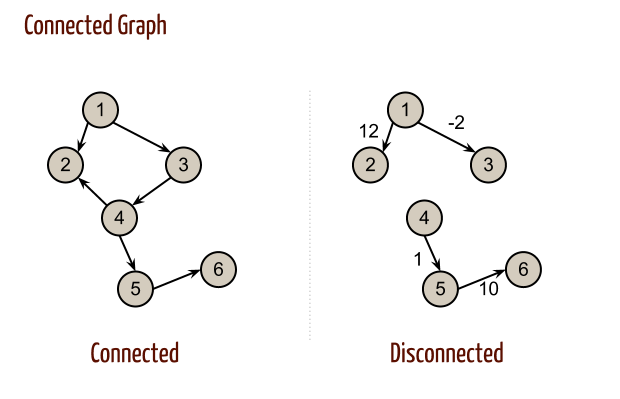
\includegraphics[scale=0.3]{connectedgraph.png}\\
	\myt{Definition:} Maximal means that a graph cannot be enlarged to get another connected subgraph\\
	
	\myt{Definition:} Let X be a subset of V(G). The \underline{cut induced by X} is the set of edges with one end in X and one end is V(G)/X\\
	
	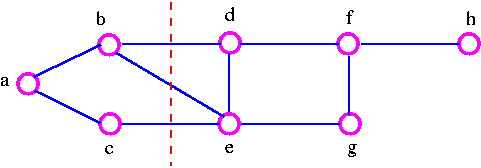
\includegraphics[scale=0.5]{cut.png}
	
	X = \{a,b,c\}\\
	The cut induced by X is \{bd,be,ce\}\\
	
	\myt{Theorem:} A graph G is disconnected if an d only if there exists a non-empty proper subset x of V(G) where the cut induced by X is empty.\\
	
	Proof: $\implies$\\
	IF G is disconnected, then it has at least two components. Let H be one component, hten V(H) is non-empty (by definition) and a proper subset (there is another component) of V(G). IF there is an edge in the cut induced by V(H) then H can be enlarged to get a larger connected subgraph which is not possible since H is maximal. So the cut induced by V(H) is empty.\\
	
	$\impliedby$\\
	Let X be a non-empty proper subset of V(G) with an empty cut. so there exists u $\in$ X and V $\in$ X that are vertices of G. Suppose there is a u,v-path $v_0,v_1....v_k$ where $v_0 = u_1, v_k = v$. We see that $v_0$ is in X and that $V_k$ is not in X. So there exists i such that $v_0, v_1... v_i \in X$ but $v_{i+1} \notin$ X. Then $v_i, v_{i+1}$ is an edge that the cut induced by X, which is not possible. So, no u,v path exists and G is disconnected.\\
	
	\subsection*{Disconnected Example:}
	Let $G_n$ be the graph where vertices are binary strings of length n, and two strings are adjacent if and only if they differe by exactly 2 bits\\
	
	Claim: \\
	$G_n$ is disconnected for all n. Let x be the number of 0's. X is a non-empty proper subset of V($G_n$). Suppose st is any edge where $s \in X$. Since we change 2 bits of S to get to T the number of 0's has the same partiy in s and t so $t \in x$ and the cut induced by x is empty. So $G_n$ is disconnected\\
	
	\section*{Euler Tours}
	
	\myt{Deftition:} A Euler Tour is a closed walk which uses every edge of the graph exactly once.\\
	
	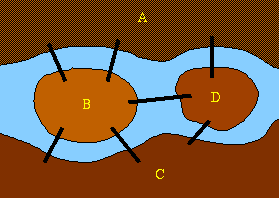
\includegraphics[scale=0.5]{eulertour.png}
	
	
	
\end{document}
